% Chapter 1

\chapter{Conclusions} % Main chapter title

\label{cha:conclusions} % For referencing the chapter elsewhere, use \ref{Chapter1} 

\lhead{Chapter 8. \emph{Conclusions}} % This is for the header on each page - perhaps a shortened title

%----------------------------------------------------------------------------------------

This final Chapter is intended to summarise and conclude the work that has been carried out in this thesis. A number of systems have been studied extensively, including S$^{9+}$, Ar$^{2+}$ and Co$^{2+}$. All three systems are useful in various astrophysical plasmas, and the lighter systems also help to test the latest up-to-date versions of the $R$-matrix computer codes. We are therefore able to determine an applicable set of atomic data for the Fe-peaks of Co$^{+}$ and Co$^{2+}$, which include energy eigenvalues, transition probabilities, photoionization cross-sections and electron-impact excitation cross-sections. A number of minor computer codes have also been introduced to assist in the maintenance and analysis stage for these large sets of data.

In particular, the {\sc bp} and {\sc darc} suites of computer codes detailed in Chapter \ref{cha:rmatrix} have been considered here. These calculations now constitute the largest and most complete to date for these individual species. To conduct a thorough evaluation of this work, we split this final Chapter into three Sections which correspond to each species, and lastly, we report on future work that has stemmed from the work presented.

\newpage

\section{Sulphur}
S$^{9+}$ is the first ion stage that we have considered in Chapter \ref{cha:sulphur}. It has been a necessary investigation for establishing the {\sc bp} suite of codes, and also because of its astrophysical importance.

The target wavefunctions were obtained by including 9 configurations in the close-coupling expansion, where the $n=3$ orbitals have been optimized on their lowest lying quartet states by implementing the computer package {\sc civ3}. Correlation effects were included in the wavefunction through the configuration-interaction method, ensuring our basis set can accurately describe the photoionization process. We were able to compare these 215 $J\pi$ fine-structure energy levels from a number of other theoretical work performed by \citet{0004-637X-762-1-53}, \citet{2003ADNDT..85..169B}, and \citet{2004ADNDT..87....1F} and also with the observational compilation from NIST \citep{1990JPCRD..19..821M}. This provided an initial measure of the accuracy obtained for the target wavefunction description. These theoretical works publish energy values, but have considered the electron-impact excitation process, and therefore we have published the first $R$-matrix evaluation for the photoionization of S$^{8+}$. We also present comparisons with the only other calculation available, those contained in the OPEN-ADAS database. The results are shown in Figures \ref{fig:sul_target}, \ref{fig:sul_adas2e}, \ref{fig:sul_adas1e} and \ref{fig:sul_adas0e} and exhibit excellent agreement for the majority of transitions considered.

The {\sc qb} code based on the theory in Section \ref{sec:rmat_qb} has also been applied in order to identify major resonance series within the lowest eight target thresholds. However, there is no other work that we can compare with, so these results are presented for the first time.
 
Due to the convergence between this $R$-matrix evaluation and the OPEN-ADAS dataset, we are confident in our results and the work has been published in \citet{2015JPhB...48o5204T}.

\section{Argon}
Secondly, we provide an extensive survey of Ar$^{2+}$ in Chapter \ref{cha:argon}. Two different $R$-matrix codes were used here, and both sets of results were compared with other theoretical and experimental work. 

Two different models were considered from {\sc civ3} and {\sc grasp0}, and have been summarized in Tables \ref{tab:arg_ci} and \ref{tab:arg_calculations}. The energy eigenvalues from the corresponding $R$-matrix calculations \textit{PBP3} and \textit{DARC3} are in excellent agreement with other results which includes the electron-impact excitation calculations by \citet{2009A&A...500.1253M} and \citet{2012EPJD...66...84S}, and also with NIST \citep{2010JPCRD..39c3101S}. We have also looked at the inclusion of configuration-interaction and its importance in the comparison of oscillator strengths. They are compared with the existing work by \citet{2006ADNDT..92..607F}. and \citet{2001JQSRT..69..171L}, where we achieve excellent conformity.

The agreement concerning the valence shell photoionization is apparent in Figures \ref{fig:arg_ground} and \ref{fig:arg_zoom}. We have considered the {\sc bp} computer package, with an orbital basis set of 124 levels from {\sc civ3}, and this is our \textit{PBP3} model. The second calculation has been performed with {\sc darc}, including 512 levels using {\sc grasp0} orbitals, and this is our \textit{DARC3} model. 

It has also been possible to compare with \citet{2012PhRvA..85d3408B} to investigate the L$_2$-shell photoionization process by including an additional ten `hole' states from the 2p$^5$3s$^2$3p$^5$ configuration. The cross-sections have been convoluted with a Gaussian profile of 140 meV at full-width half-maximum to replicate experimental resolution. We have shown the contributions from the valence shell and direct `2p' photoionization in Figure \ref{fig:arg_l-shell} to compare the different ionization modes from experiment. This is due to the autoionizing states decaying via the Auger process which occurs on a timescale quicker than that of the time of flight of the ion. We also provide the calculations from {\sc mchf} and {\sc opas} in Figure \ref{fig:arg_l-shell-big} to show the extent of the agreement. Since these features are not completely isolated, it is difficult to determine the composition of the initial Ar$^+$ states in the experiment, and we therefore adopt a typical statistical weighting for our comparison. However, the level separations of these additional ten levels determined from the $R$-matrix calculation results in excellent energy positions of the resonant states between experiment and theory.

We have failed to identify these autoionizing bound states in this region with the {\sc qb} code for the \textit{DARC3} model, as it has not been possible to run this serial code with such a large $R$-matrix calculation. This concludes our detailed study of Ar$^+$ which is the largest to date, and the results have been published in \citet{2016MNRAS.456..366T}.

\section{Cobalt}
This third and final Section concerns the astrophysical important ions of cobalt considered in Chapter \ref{cha:cobalt}. We have implemented the {\sc darc} computer codes, complementary to {\sc grasp0} for the Co$^{2+}$ orbital basis set description. Few data are available to compare with, and recently only one $R$-matrix calculation has been performed using the {\sc autostructure} and {\sc bp} suite of codes.

We initially look at the comparison of energy levels with \citet{1985aeli.book.....S} and the lowest 15 from the $R$-matrix calculation by \citet{2016MNRAS.tmp..556S}. There is clear agreement between these results in Table \ref{tab:co_energy}, but differences between the higher 3d$^7$ states can be quite significant. During PSTG3R, we have adjusted our target thresholds to coincide with \citet{1985aeli.book.....S}, and therefore a careful treatment of all 292 levels must be considered. We have also compared our $A$-values from {\sc grasp0} with \citet{2016MNRAS.tmp..556S}, \citet{2016A&A...585A.121F}, and \citet{1984ApJ...277..435H}, where modelling codes have implemented the latter until recently. We believe that the results provided by \citet{2016A&A...585A.121F} are the most accurate, due to the complexity in the structure calculation.

Previous work conducted by \citet{1979ApJS...40..815R}, \citet{1993ADNDT..55..233V}, and \citet{2015JPhB...48n4014F}, have presented approximate photoionization cross-sections that we can compare with. These results are provided for the statistically weighted ground and excited initial states of Co$^+$ in Figures \ref{fig:co_ground} and \ref{fig:co_excited}. Partial recombination rates defined in equation (\ref{eq:spe_partialrate}) can be calculated by considering the partial cross-sections from each initial bound state. Figure \ref{fig:co_rates} shows the recombination rates obtained by applying equations (\ref{eq:spe_partialrate}), (\ref{eq:spe_milne}), and (\ref{eq:spe_formalrate}) from the three lowest Co$^+$ initial bound states to the $^4$F$_{9/2}$ final state.

For the electron-impact excitation process, all partial waves up to $J=13$ and top-up to $J=38$ have been included. We compute Maxwellian averaged collision strengths by applying equation \ref{eq:rmat_ups}, for temperatures $3,800 \leq T \leq 40,000$ in K and the effective collision strengths are provided in an \textit{adf04} file. Also included are energy eigenvalues and $A$-values, which are $\Delta E$ shifted according to equation (\ref{eq:many_ascale}). The effective collision strengths are compared directly with the work of \citet{2016MNRAS.tmp..556S} for select transitions. There are discrepancies in Figures \ref{fig:co_coll_infra1}, \ref{fig:co_coll_infra2}, and \ref{fig:co_coll_infra3} between the low lying levels, but excellent agreement can be seen from Figure \ref{fig:co_coll_5to7} for other transitions. 

We have also investigated features of the computer code {\sc collr-v1.0} by implementing the \textit{adf04} file including Co$^{2+}$. The agreement for low (equation (\ref{eq:spe_coronal})) and high (equation (\ref{eq:spe_lte})) density regimes, i.e. coronal equilibrium and LTE agree extremely well for all transitions considered, and one example is provided in Figure \ref{fig:co_consttemp}. Line ratios defined by equation (\ref{eq:spe_lratio}) have also been investigated here which provides useful density and tempteraure diagnostics and can be seen from Figures \ref{fig:co_consttemp}, and \ref{fig:co_constdens}.

We conclude this Section by proposing one further investigation of how the various atomic data discussed above has an effect on these line ratios. This work has also recently been submitted for publication to Monthly Notices of the Royal Astronomical Society.

\section{Future work - A study of neutral nickel}
We have included this final Section to detail the additional work that is currently in progress. Preliminary results have been obtained, and the analysis has now begun. The majority of this thesis has focused on the process of photoionization and its importance to the astrophysics community, and on low ionization species of cobalt. Iron has received a large amount of attention due to its high abundance and challenging electronic structure, and for this reason we aim to provide atomic data concerning systems of nickel and additional ionization stages of cobalt. This will instigate further calculations in the future, and benchmark these data sets for astrophysical modelling.

Low ionization stages of nickel, including neutral nickel, are observed in many astrophysical objects. These include absorption and emission lines in SN remnants \citep{1980ApJ...242.1023F}, the Orion nebula \citep{1975ApJ...199L..43G}, $\eta$-Carinae \citep{1967MNRAS.135...51T}, and gaseous nebula \citep{1995A&A...294..555L}. Theoretical quantities have been determined to accommodate these multiple observations, and include transition probabilities of Ni and Ni$^+$ \citep{1996A&AS..119...99Q}, photoionization cross-sections of Ni$^+$ \citep{1999A&AS..137..529B}, and nebular investigations \citep{1982A&A...110..295N}. Since nickel is the heaviest element in the decay path of SNe, there are also many publications in this field of astrophysics. The mass of ejected Ni$^{56}$ can often be inferred from the bolometric light curves, such as in SN 2004A by \citet{2006MNRAS.369.1303H}, and strong lines are observed from other SNe \citep{1990MNRAS.242..669S, 2003MNRAS.346...97N, 2006MNRAS.369.1780V}.

In this Section we compute the photoionization cross-sections for neutral nickel. This is described by the following process,
\begin{equation}\label{eq:conc_photo}
h\nu + {\rm Ni} \rightarrow {\rm Ni}^{+}+e^-.
\end{equation}
According to NIST \cite{1985aeli.book.....S}, there are five unique electronic configurations, 3d$^8$4s$^2$, 3d$^9$4s, 3d$^9$4p, 3d$^{10}$, and 3d$^8$4s4p between 0 - 3.5 eV. Since the wavefunctions are constructed from the target ion Ni$^+$, we must be extremely confident that these bound states can also be accurately represented. 

\begin{table}[hbt]
\footnotesize
\begin{center}
\begin{tabular}{@{}        c c c c         c c c c c        @{}}
\toprule
\multicolumn{1}{c}{Index} & \multicolumn{1}{c}{Config.} & \multicolumn{1}{c}{Term} & \multicolumn{1}{c}{\textit{S\&C}} & \multicolumn{1}{c}{\textit{Present}} & \multicolumn{1}{c}{2J} & \multicolumn{1}{c}{\textit{S\&C}} & \multicolumn{1}{c}{\textit{Present}} & \multicolumn{1}{c}{\textit{Cassidy}} \\  

\toprule
                                            
                                           
\multicolumn{1}{c}{1} &  3d$^9$  & $^2$D  & 0.0000   & 0.0000 &  5 &   0.0000  &  0.0000 &  0.0000\\
\multicolumn{1}{c}{2} &  3d$^8$4s  &               &  &   &   3 &   0.1868  & 0.2374 &  0.1968\\
\multicolumn{1}{c}{3} &  3d$^8$4s  & $^4$F  &   1.0851  & 1.1817  &  9 &   1.0407 &  0.9781 &  1.2654\\
\multicolumn{1}{c}{4} &  3d$^8$4s  &               &    &   &  7 &   1.1568   & 1.1141 &  1.3865\\
\multicolumn{1}{c}{5} &  3d$^8$4s  &               &    &  &  5 &  1.2542   & 1.2319 &  1.4864\\
\multicolumn{1}{c}{6} &  3d$^8$4s  &               &    &   &  3 &   1.3222  &  1.3153 &  1.5561\\
\multicolumn{1}{c}{7} &  3d$^8$4s  & $^2$F  &  1.6821  & 1.7730  &  7 &  1.6800  &  1.6656 &  1.9805\\
\multicolumn{1}{c}{8} &  3d$^8$4s  &                &   & &  5 &   1.8592 &  1.8830 &  2.1662\\
\multicolumn{1}{c}{9} &  3d$^8$4s  & $^4$P  &  2.8955     &  3.5621 &  5 &  2.8651 &  3.4476 &  3.5006\\
\multicolumn{1}{c}{10} &  3d$^8$4s &                &   &  &  3 &   3.0733  &  3.4955 &  3.4816\\
\multicolumn{1}{c}{11} &  3d$^8$4s  &                &    &   &  1 &   3.0793  &  3.8094 & 3.4964\\
\multicolumn{1}{c}{12} &  3d$^8$4s  & $^2$D  &  2.9679    &  3.7874 &  3 &    2.9504  & 3.7807 &  3.3203\\
\multicolumn{1}{c}{13} &  3d$^8$4s  &                 &    &   &  5 &    3.1041  &  3.7703 &  3.2483\\
\multicolumn{1}{c}{14} &  3d$^8$4s  & $^2$P  & 3.5512 &  4.3949 &  3 &   3.6043  &  4.3634 &  4.0867\\
\multicolumn{1}{c}{15} &  3d$^8$4s  &                  &    &   &  1 &   3.6691   &  4.4372 &  4.1522\\
\multicolumn{1}{c}{16} &  3d$^8$4s  & $^2$G  & 3.9560   & 4.7829  &  9 &  4.0294 &  4.7435 &  4.5276\\
\multicolumn{1}{c}{17} &  3d$^8$4s  &                  &   &  &  7 &  4.0324  &  4.7439 &  4.5313 \\
\multicolumn{1}{c}{18} &  3d$^7$4s$^2$  &  $^4$F  &  6.3934    & 6.5570 &  9 &  6.3288  &  6.2418 &  7.4645\\
\multicolumn{1}{c}{19} &  3d$^7$4s$^2$  &                  &    &   &  7 &  6.4727 &  6.3958 & 7.6100\\
\multicolumn{1}{c}{20} &  3d$^7$4s$^2$  &                  &  &   &  5 &  6.5759  &  6.5079 &  7.7148\\
\multicolumn{1}{c}{21} &  3d$^7$4s$^2$  &                  &    &   &  3 &    6.6457  &  6.5844 &  7.7856\\
\multicolumn{1}{c}{22} &  3d$^8$4p  &  $^4$D$^{\rm o}$ &   6.4455   & 6.6966  &  7 & 6.3924   &  6.6205 & 6.5374\\
\multicolumn{1}{c}{23} &  3d$^8$4p  &                  &    &  &  5 &   6.5387   &  6.8147 &  6.6843\\
\multicolumn{1}{c}{24} &  3d$^8$4p  &                  &    &   &  3 &   6.6498  &  6.9610 &  6.7939\\
\multicolumn{1}{c}{25} &  3d$^8$4p  &                  &    &   &  1 &    6.7170 & 7.0511 &  6.8597\\
         
\bottomrule
 \end{tabular}
  \caption{Lowest energy values for 25 levels, and 9 terms of Ni$^{+}$. Comparisons are between the \textit{Present} $R$-matrix with pseudo-state calculation, \textit{S\&C} from the NIST database \citep{1985aeli.book.....S}, and the results from the electron-impact excitation calculation performed by \citet{2010A&A...513A..55C}  \label{tab:ni_energy}}
 \end{center}
\end{table}

The first attempt at a calculation is a follow up to work performed by \citet{clarathesis}. The electron-impact excitation process has been investigated for Ni$^+$ \citep{2010A&A...513A..55C, 2011ApJ...738....5C} by considering a basis set involving STO's generated from {\sc civ3} which includes spectroscopic orbitals up to $4p$ and a pseudo orbital $\bar{4d}$. It is then possible to incorporate this data into the {\sc bp} suite of codes and include the same description for the Ni$^+$ target.

%
%%
%%%
%%%%
\begin{figure}[h]
\centering
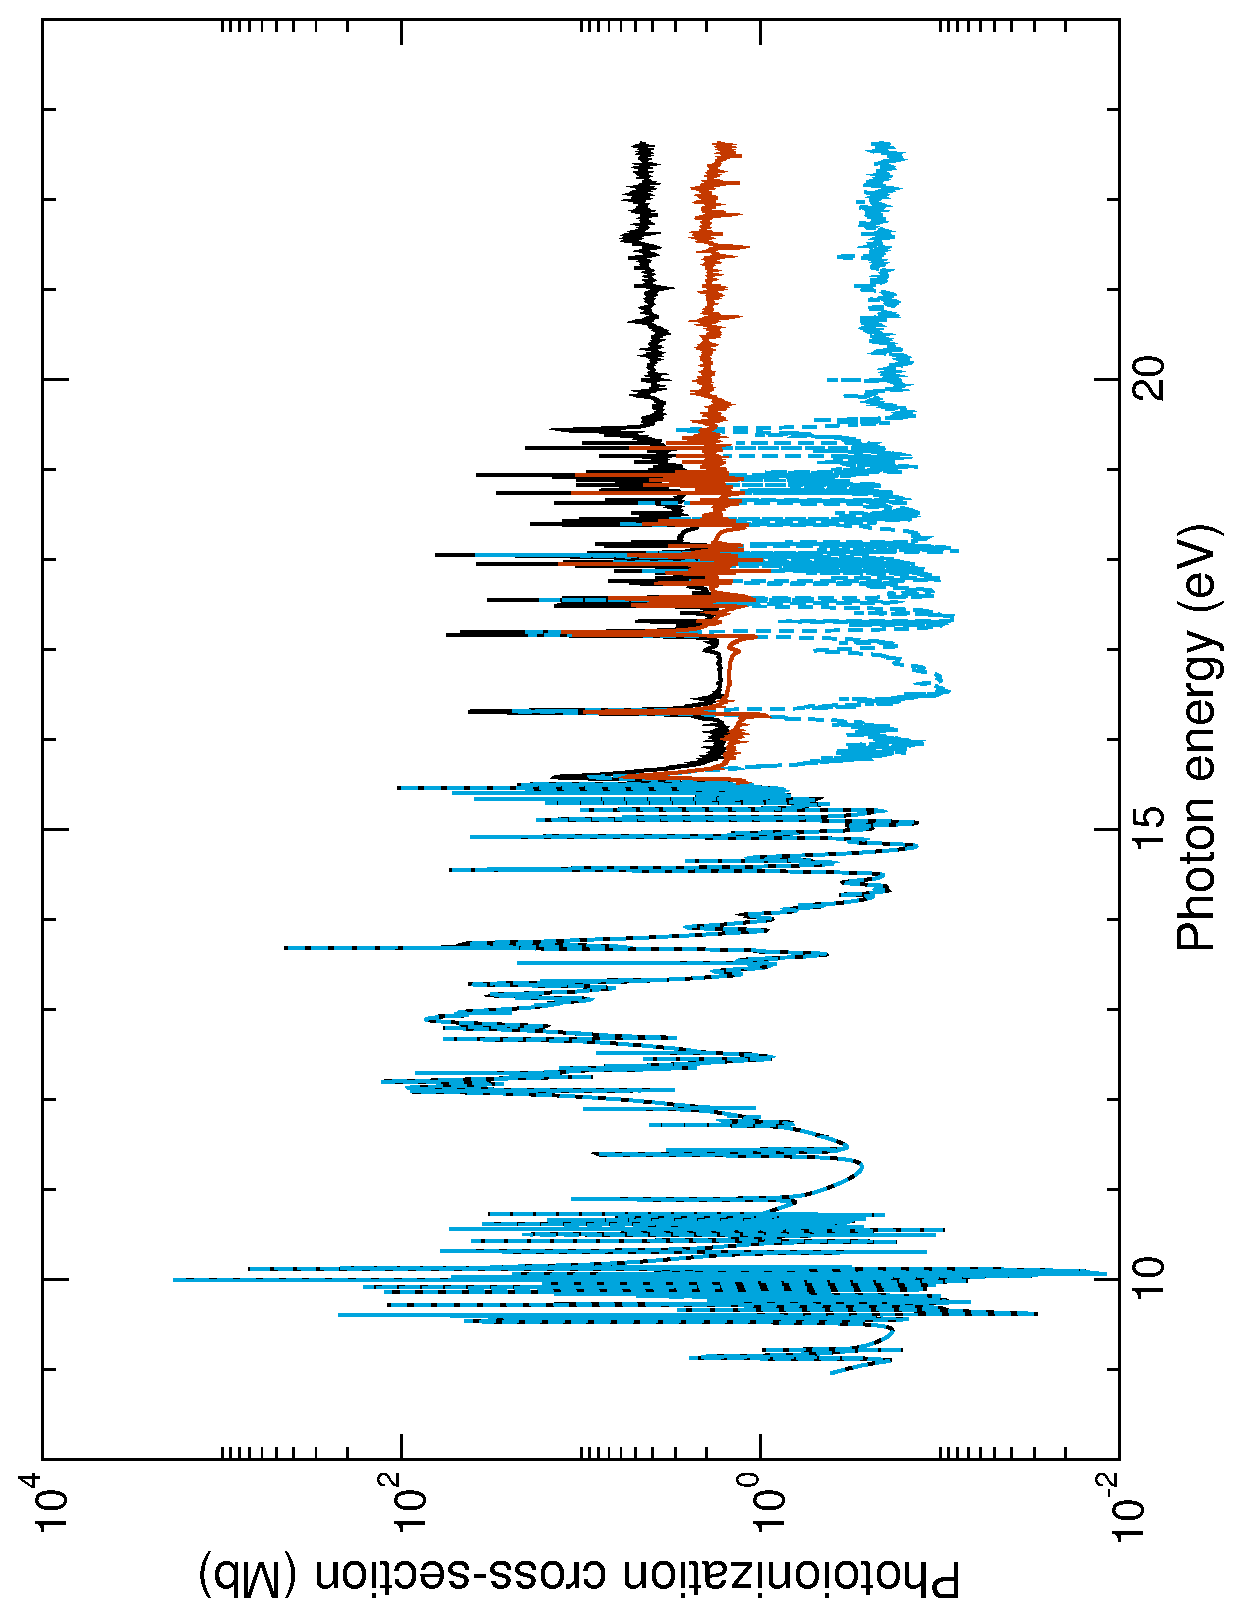
\includegraphics[scale=0.5,angle=-90]{Figures/Conclusions/ni_rmps.eps}
\caption{The photoionization cross-section in Mb presented as a function of the photon energy in eV. The solid black curve is the total cross-section from the initial ground state 3d$^8$4s$^2$ $^3$F to all allowed final states, the dashed blue curve is the contribution from the first seven target terms 3d$^9$ $^2$D, 3d$^8$4s $^4$F, $^2$F, $^4$P, $^2$D, $^2$P, and $^2$G, and the orange curve is the contribution from the 3d$^7$4s$^2$ $^4$F. \label{fig:con_ground}}
\end{figure}
%%%%
%%%
%%
%

We also perform an independent calculation by using the {\sc autostructure} computer package. Spectroscopic orbitals up to $4f$ are included, and pseudo-orbitals up to $\bar{n}=12$ for $\bar{l}=0,1,2$ have also been included. These additional pseudo-states are included into the calculation to improve the target description of Ni$^+$, especially for the low-lying terms, as described by \citet{1996JPhB...29..115B}. The configurations 3p$^6$3d$^9$, 3p$^6$3d$^7$4s$^2$, 3p$^6$3d$^7$4s4p and 3p$^6$3d$^8$[4s, 4p, 4d, 4f, 5s, $\bar{n}\bar{l}]$ therefore constitute our basis set for Ni$^+$, and results in an overwhelming 597 terms in $LS\pi$ coupling. All fine-structure levels would result in an impossible task, but in a separate calculation we include the lowest 290 levels in the close-coupling expansion, which spans $\approx 20$ eV. We provide the lowest 25 levels (and 9 terms) in Table \ref{tab:ni_energy} between this calculation, and the results from NIST \citep{1985aeli.book.....S}, and also \citet{2010A&A...513A..55C} in eV. The levels presented are in excellent agreement with NIST, but with some discrepancies for the higher 3d$^8$4s (9 - 17) levels. It is worthwhile to note that for these levels, the $\%$ difference between the 3d$^7$4s$^2$ is 3.7$\%$, compared with $\approx 17\%$ from \citet{2010A&A...513A..55C}, and all levels are in energy order with those of NIST with the exception of levels 11 and 13. These 3d$^7$4s$^2$ states however are of utmost importance, as the ground state of neutral nickel is 3d$^8$4s$^2$, and this is the dominant photoionization contribution.

%
%%
%%%
%%%%
\begin{figure}[h]
\centering
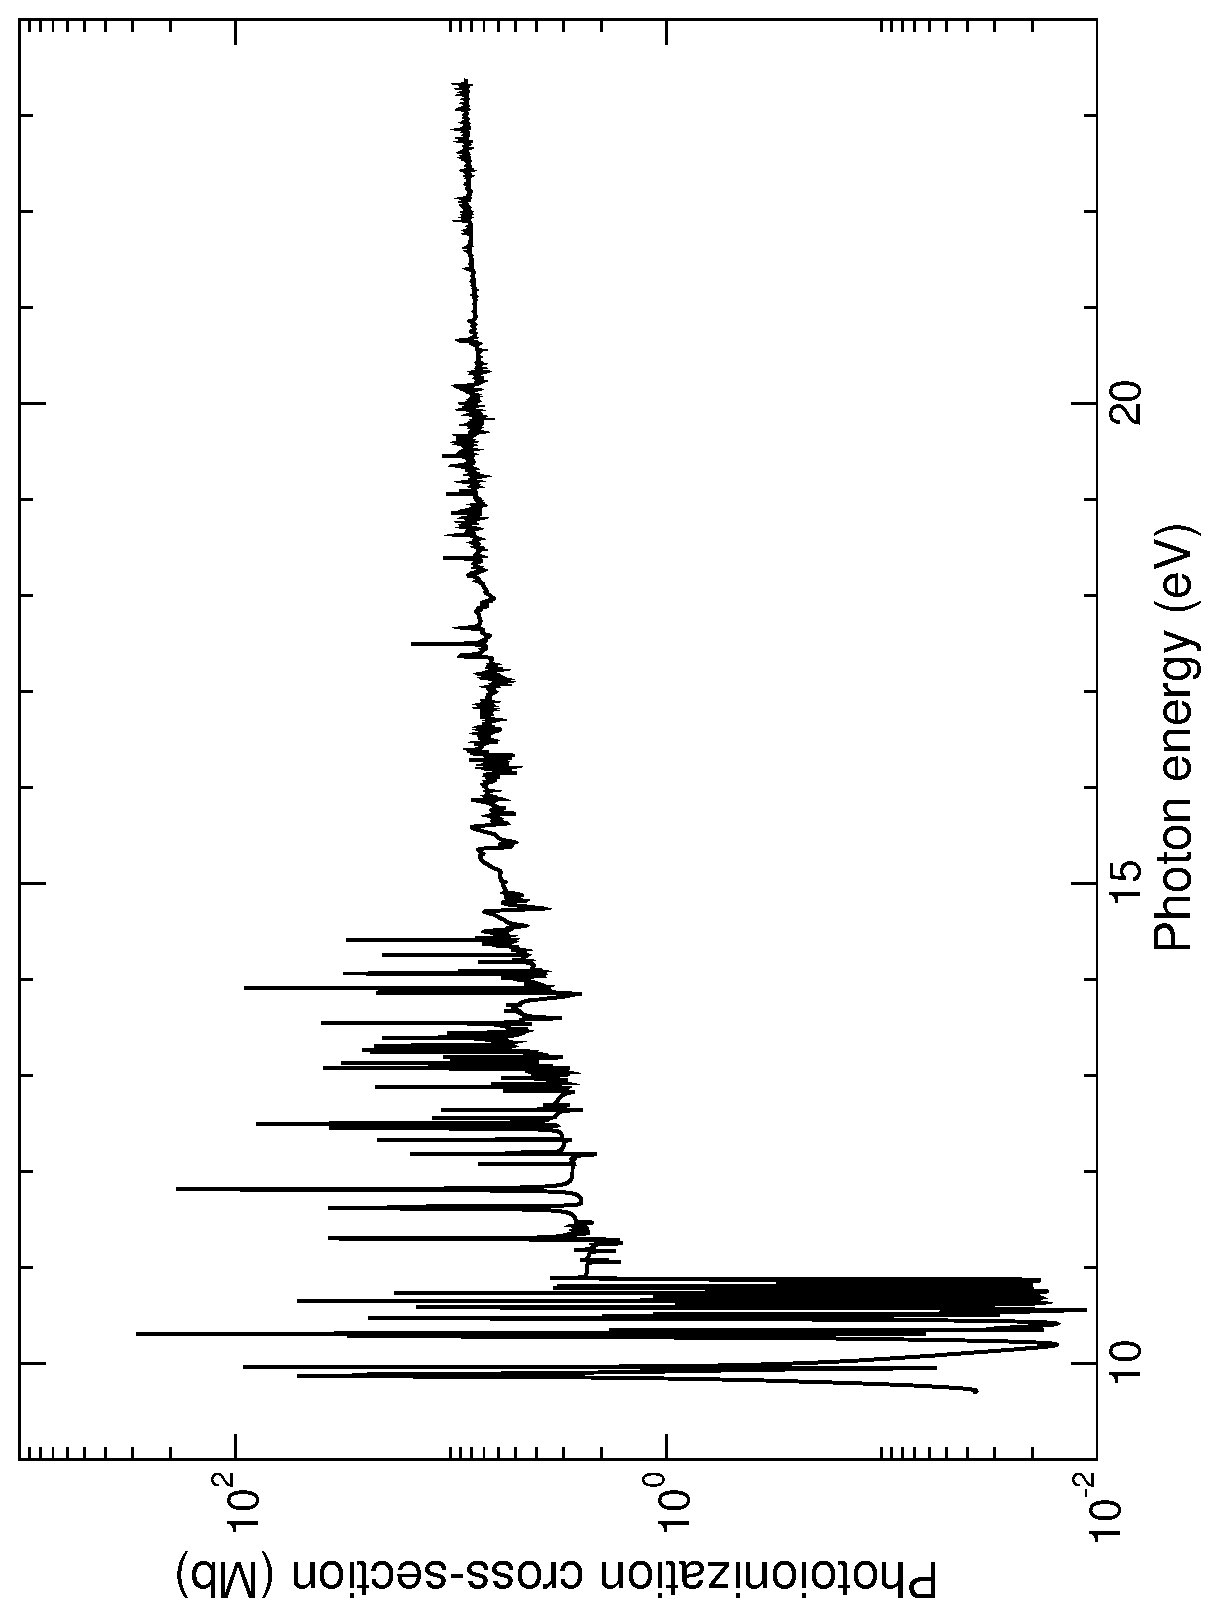
\includegraphics[scale=0.5,angle=-90]{Figures/Conclusions/ni_rmps_excited.eps}
\caption{The photoionization cross-section in Mb presented as a function of the photon energy in eV. The solid black curve is the total cross-section from the initial ground state 3d$^9$4s $^3$D to all allowed final states. \label{fig:con_excited}}
\end{figure}
%%%%
%%%
%%
%

The wavefunction description of Ni$^+$ now permits us to calculate the photoionization process defined in equation (\ref{eq:conc_photo}) by using the $R$-matrix with pseudo-states method. Due to the typical properties of SNe, we are only concerned with outer shell valence transitions, so the number of continuum orbitals is chosen to be 15 per angular momenta. In order to capture the radial distribution of the pseudo-orbitals, the $R$-matrix boundary is chosen to be 37.5 a.u. We compute up to $J=5$ odd and $J=4$ even dipole symmetries for transitions of interest.  

We present in Figure \ref{fig:con_ground} the ground state photoionization of Ni. The solid black curve represents the total cross-section from the initial $^3$F state to all allowed final states in $LS\pi$ coupling. The dashed blue curve is the contribution from the lowest seven $LS\pi$ terms 3d$^9$ $^2$D, 3d$^8$4s $^4$F, $^2$F, $^4$P, $^2$D, $^2$P, and $^2$G, and the solid orange is from the 3d$^7$4s$^2$ $^4$F term only. It is clear from the figure the importance that these 3d$^7$4s$^2$ states are in the total cross-section. We also present the photoionization cross-section from the initial 3d$^9$4s $^3$D excited state to all allowed final states in Figure \ref{fig:con_excited}. This work is therefore still in progress, and the Breit-Pauli corrections will be included to account for relativistic effects.

%----------------------------------------------------------------------------------------


